\documentclass[10pt]{article}

\usepackage[a4paper,margin=0.72in]{geometry}
\usepackage[T1]{fontenc}
\usepackage[utf8]{inputenc}
\usepackage{lmodern}
\usepackage{amsmath,amssymb}
\usepackage{booktabs}
\usepackage{array}
\usepackage{tabularx}
\usepackage{graphicx}
\usepackage{xcolor}
\usepackage{enumitem}
\usepackage{hyperref}
\usepackage{fancyhdr}
\usepackage{titlesec}
\usepackage{caption}
\usepackage{float}

\definecolor{accent}{HTML}{0F4C81}
\definecolor{softaccent}{HTML}{EAF2FB}
\definecolor{textgray}{HTML}{333333}
\definecolor{rulegray}{HTML}{AAB7C4}

\hypersetup{
    colorlinks=true,
    linkcolor=accent,
    urlcolor=accent,
    citecolor=accent
}

\setlength{\parindent}{0pt}
\setlength{\parskip}{4pt}
\setlist[itemize]{leftmargin=1.1em,itemsep=2pt,topsep=2pt}
\setlist[enumerate]{leftmargin=1.3em,itemsep=2pt,topsep=2pt}
\graphicspath{{figures/}}
\captionsetup{font=small,labelfont=bf}

\titleformat{\section}{\Large\bfseries\color{accent}}{\thesection.}{0.5em}{}
\titleformat{\subsection}{\normalsize\bfseries\color{accent}}{\thesubsection}{0.5em}{}
\titlespacing*{\section}{0pt}{8pt}{4pt}
\titlespacing*{\subsection}{0pt}{6pt}{3pt}

\pagestyle{fancy}
\fancyhf{}
\fancyhead[L]{Zak-OTFS Project Report}
\fancyhead[R]{\thepage}
\renewcommand{\headrulewidth}{0.4pt}
\renewcommand{\footrulewidth}{0pt}

\newcommand{\keybox}[1]{%
\vspace{3pt}
\noindent\fcolorbox{accent}{softaccent}{%
\parbox{\dimexpr\linewidth-2\fboxsep-2\fboxrule\relax}{#1}}
\vspace{4pt}
}

\begin{document}
\thispagestyle{empty}

\begin{titlepage}
\color{textgray}
\begin{center}
{\Large \textbf{\color{accent}Zak-OTFS Channel Estimation Project Report}}\\[0.35em]
{\large From Original Paper Reproduction to Structure-Aware Distilled Compression}\\[1.0em]

\rule{\textwidth}{1.1pt}\\[0.8em]
{\small Indian Institute of Technology Jodhpur}\\
{\small Department Project Report}\\[0.8em]
\rule{\textwidth}{1.1pt}
\end{center}

\vspace{0.8em}
\begin{minipage}[t]{0.56\textwidth}
{\bfseries Team Members}\\[0.4em]
\begin{tabular}{>{\bfseries}p{0.36\linewidth}p{0.44\linewidth}}
B23ES1023 & Mayank Sharma\\
B23ES1029 & Rohit Kumar Mourya\\
B23ES1017 & Jyotiraditya Singh Rathore\\
B23ES1021 & Madhav\\
B23ES1014 & Dikshant Jha\\
\end{tabular}

\vspace{1.0em}
\keybox{\textbf{Report Scope.} This report explains the original Zak-OTFS paper, our independent baseline reimplementation, the structural novelty we added, and the final comparison between the original method, our baseline, and our distilled Lite models.}

\vspace{0.8em}
{\bfseries Deliverables Covered}
\begin{itemize}
    \item Original-paper explanation in clear engineering language
    \item Baseline reimplementation and comparison with the published method
    \item Novelty: physics-induced support compressibility and distilled Lite-M model
    \item Quantitative comparison using the validated results available in our pipeline
    \item Team contribution split
\end{itemize}
\end{minipage}\hfill
\begin{minipage}[t]{0.40\textwidth}
    \centering
    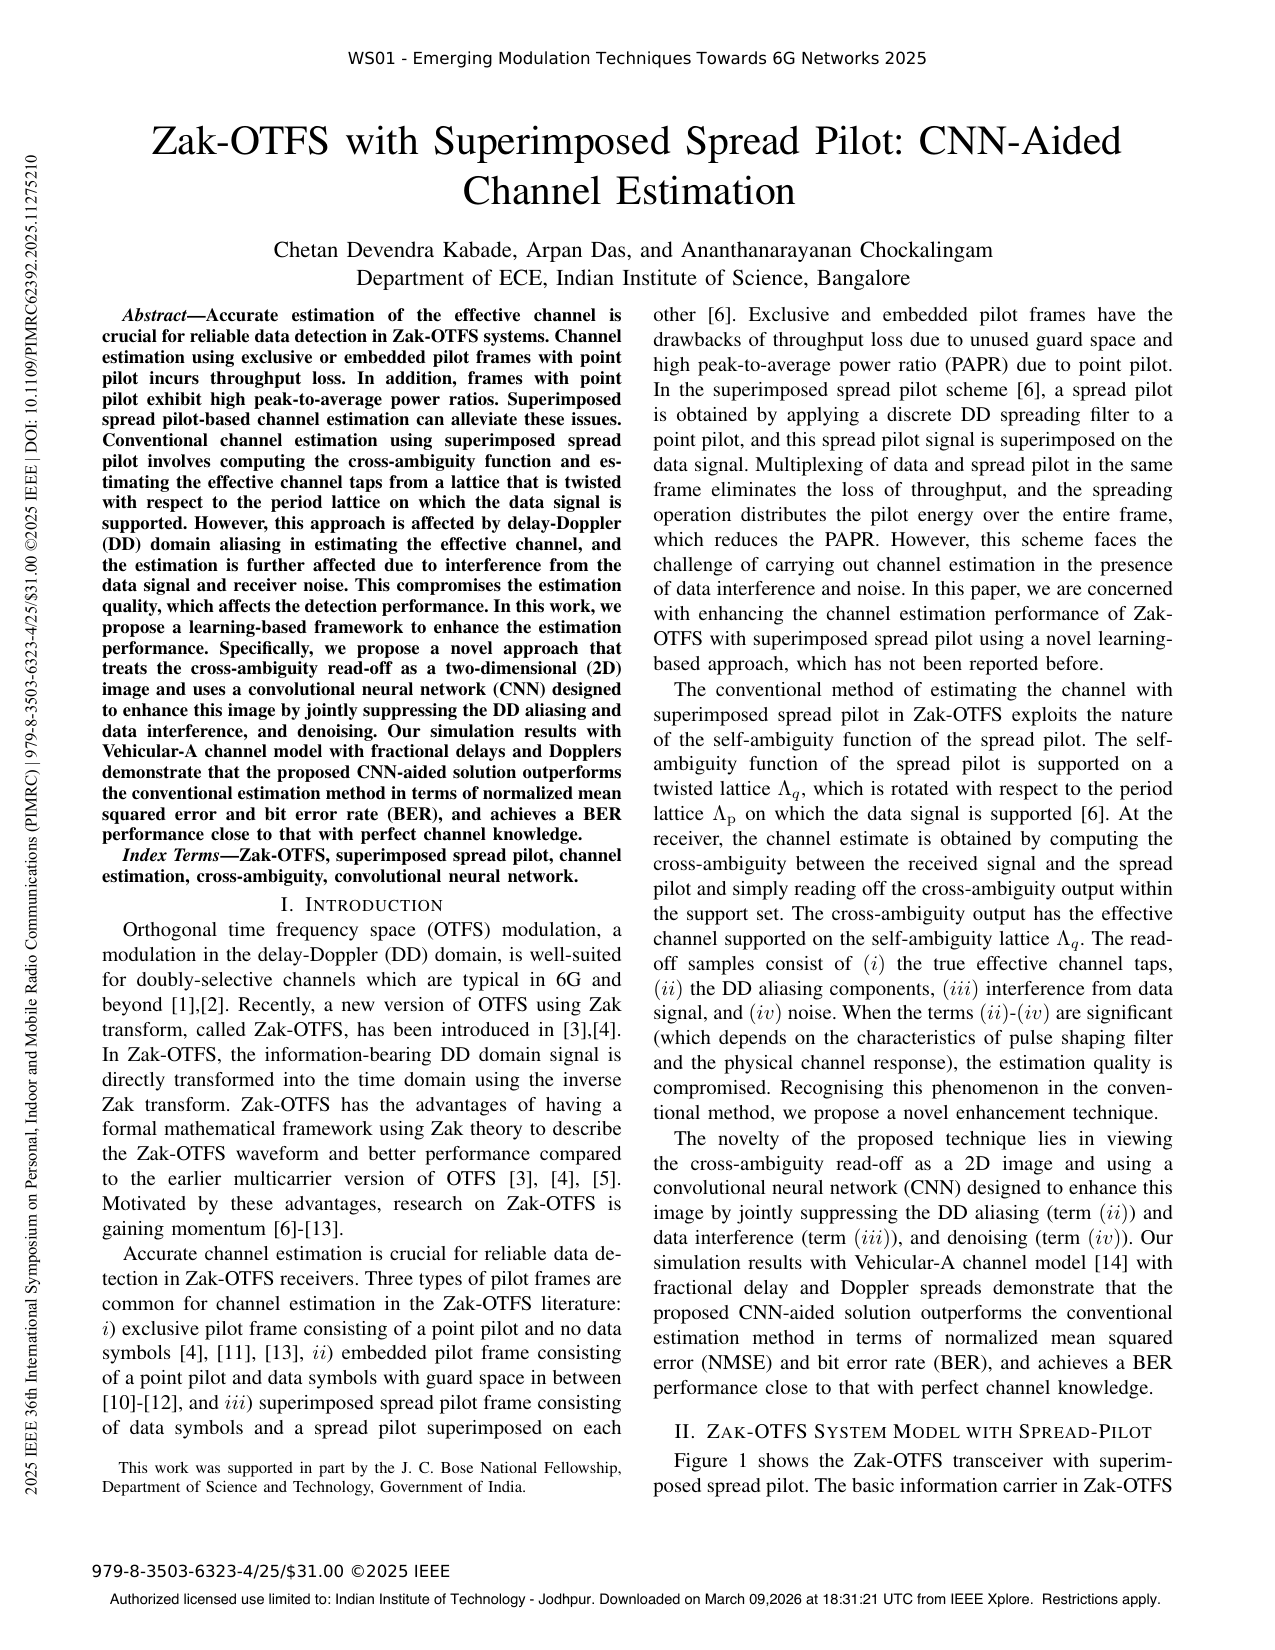
\includegraphics[width=\linewidth]{original_paper_cover.png}\\[0.4em]
    {\footnotesize First page of the original PIMRC 2025 paper that motivated this project.}
\end{minipage}

\vfill
\begin{center}
{\small Prepared from the reproduced Zak-OTFS baseline, the distilled-student extension, and the final structural-compressibility analysis.}
\end{center}
\end{titlepage}

\section{Original Paper: What It Does and Why It Matters}

The original paper, ``Zak-OTFS with Superimposed Spread Pilot CNN-Aided Channel Estimation,'' studies channel estimation for Zak-transform-based OTFS in a highly time-varying wireless setting. Its key engineering idea is that a spread pilot can be superimposed on the delay-Doppler (DD) grid without the guard-band overhead used in earlier embedded-pilot OTFS schemes. The receiver reads out a compact twisted-support channel image from the cross-ambiguity response and then refines that image using a convolutional neural network (CNN).

The paper matters for two reasons. First, it targets a physically meaningful high-mobility regime where accurate DD-domain channel estimation is difficult. Second, it proposes a CNN-aided improvement over the conventional read-off estimate without changing the overall Zak-OTFS detector structure. In other words, the learned part sits at a very important junction: if the support image is improved, both pilot cancellation and downstream data detection improve.

\keybox{\textbf{Original paper in one line.} The published method treats the twisted-support DD channel estimate as a small complex image and uses a CNN to denoise it before LMMSE detection.}

At a high level, the original pipeline is:
\begin{enumerate}
    \item Superimpose data and a spread pilot in the Zak-OTFS DD grid.
    \item Pass the signal through a sparse Vehicular-A channel with fractional delay and Doppler shifts.
    \item Read off a compact support-domain channel image from the pilot response.
    \item Use a CNN to refine the noisy support image.
    \item Re-embed the refined estimate into the DD grid and perform pilot cancellation plus LMMSE data detection.
\end{enumerate}

The original paper reports that its CNN-aided estimate approaches the perfect-CSI reference under its published evaluation setting. However, no official code accompanied the paper, so any later implementation effort must be framed as a careful reimplementation rather than a byte-for-byte reproduction of the authors' internal code.

\section{Our Baseline: What We Rebuilt, Why We Rebuilt It, and How It Compares}

\subsection{What We Rebuilt}

Because the original paper did not provide an official repository, we rebuilt the full workflow ourselves:
\begin{itemize}
    \item Zak-OTFS DD-grid construction and spread-pilot generation
    \item Vehicular-A channel simulation with fractional delay-Doppler shifts
    \item Cross-ambiguity-based support read-off
    \item The published CNN architecture for support-image refinement
    \item Pilot cancellation and LMMSE detection
\end{itemize}

The most important baseline choice was to preserve the \emph{published estimator design}: the same four-layer CNN, large-kernel image-processing view of the support crop, and the same overall inference path from support estimation to detection.

\subsection{Why the Baseline Was Necessary}

The baseline is not just background code. It is the foundation that makes the later novelty defensible. Without it, any compact model would have no trustworthy teacher, no fair evaluation path, and no way to separate true novelty from implementation noise. The baseline also forced us to document where the original paper was underspecified, especially around the effective-channel construction and matched-filter discretization.

\subsection{How Our Baseline Compares with the Original Paper}

\begin{table}[H]
\centering
\caption{Original paper vs.\ our baseline reimplementation.}
\begin{tabularx}{\linewidth}{>{\bfseries}p{0.19\linewidth}X X}
\toprule
Aspect & Original paper & Our baseline \\
\midrule
Code availability & No official public repository & Full independent implementation \\
Estimator & CNN-aided support-image denoiser & Same estimator structure reproduced \\
CNN size & Large four-layer CNN & Same verified architecture: 245,473 params \\
Physics path & Described in paper & Fully implemented end-to-end \\
Detector & Pilot cancellation + LMMSE & Same detection path retained \\
Numerical comparability & Published results only & Internally consistent within our implementation, but not claimed as exact author-code parity \\
\bottomrule
\end{tabularx}
\end{table}

Our baseline is faithful in \emph{structure} rather than guaranteed identical in every hidden implementation detail. That distinction matters. It means we can compare teacher and student models honestly inside our own pipeline, while avoiding the unsafe claim that we exactly reproduced the unpublished author code.

\section{Novelty We Added: Structural Compressibility + Distilled Lite Models}

\subsection{The Core Insight}

Our novelty is \textbf{not} merely ``we compressed a CNN.'' The stronger insight is that the Zak-OTFS support-domain channel image is structurally compressible for physical reasons.

Under the fast effective-channel model used in our implementation, the true support image can be written as a deterministic chirp multiplied by a sum of path-wise separable delay and Doppler atoms. After removing the known support chirp, the dechirped support image becomes a sum of outer products. With $P$ physical paths, this means the rank is bounded by $P$.

\keybox{\textbf{Main novelty statement.} The distilled student works well because the Zak-OTFS support image is not a generic image-denoising problem. After dechirping, the target lies on a low-dimensional physics-induced manifold.}

This changes the interpretation of the whole project:
\begin{itemize}
    \item The teacher CNN is strong, but it is solving a structured denoising problem.
    \item A compact student can imitate that behavior because the target geometry is already constrained.
    \item Distillation is therefore justified by physics-induced compressibility, not just by trial-and-error model shrinking.
\end{itemize}

\subsection{Evidence for the Structural Claim}

We validated this in three ways:
\begin{enumerate}
    \item \textbf{Exact fast-model structure.} After dechirping, the true support image has negligible singular-value tail energy beyond the path count $P=6$.
    \item \textbf{Reference-model support.} The slower reference construction does not admit the same clean symbolic factorization, but numerically it still shows sharply concentrated singular spectra.
    \item \textbf{Simple non-learned SVD baseline.} A dechirp-plus-truncated-SVD projection already recovers much of the conventional denoising gain, which shows that projection toward a low-rank manifold is doing real work.
\end{enumerate}

\begin{figure}[H]
    \centering
    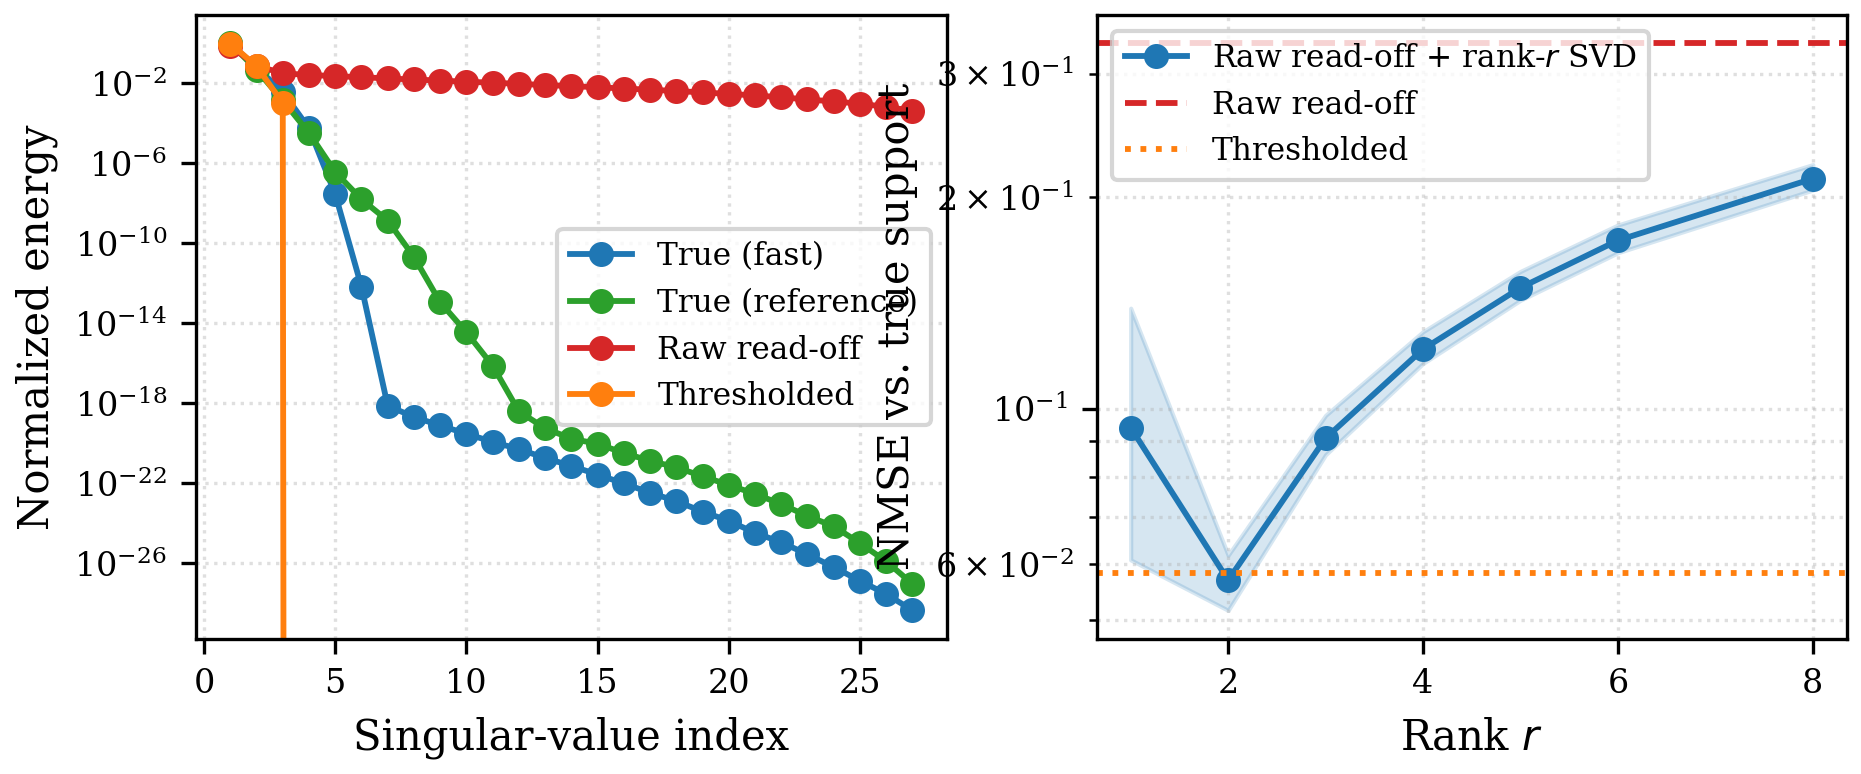
\includegraphics[width=0.92\linewidth]{support_structure_overview.png}
    \caption{Structural-compressibility evidence. The dechirped true support image is sharply concentrated, while the raw read-off observation has a much heavier singular tail. A simple low-rank projection already recovers much of the denoising gain.}
\end{figure}

\subsection{The Distilled Lite Models}

After establishing that the task itself is compressible, we distilled the 245,473-parameter teacher into three compact students:
\begin{itemize}
    \item \textbf{Lite-L:} 40,049 parameters
    \item \textbf{Lite-M:} 22,789 parameters
    \item \textbf{Lite-S:} 6,137 parameters
\end{itemize}

The student loss combines teacher imitation and ground-truth supervision, so the compact models inherit the teacher's denoising behavior while staying tied to the true support-domain channel. Among the three, \textbf{Lite-M emerged as the best overall tradeoff point}.

\section{Results and Clear Comparisons}

\subsection{Original vs.\ Baseline vs.\ Our Novelty}

The comparison must be stated carefully:
\begin{itemize}
    \item \textbf{Original paper:} introduces the CNN-aided Zak-OTFS estimator and reports strong gains versus the conventional estimator.
    \item \textbf{Our baseline:} independently reconstructs that pipeline with the same overall estimator design and uses it as the teacher model.
    \item \textbf{Our novelty:} explains why compression should work and realizes that idea through a compact distilled Lite-M student.
\end{itemize}

\begin{table}[H]
\centering
\caption{Original paper, our baseline, and our novelty compared.}
\begin{tabularx}{\linewidth}{>{\bfseries}p{0.20\linewidth}X X X}
\toprule
Aspect & Original paper & Our baseline & Our novelty \\
\midrule
Main message & CNN helps DD support estimation & Reproduce the full pipeline faithfully & Explain compressibility and exploit it through distillation \\
Code & Not publicly available & Fully rebuilt by us & Built on the verified baseline \\
Explainability & Limited structural explanation & Strong engineering grounding & Physics-induced low-dimensional explanation \\
Compact model & No & No & Yes, Lite-L / Lite-M / Lite-S \\
Headline model & CNN estimator & Teacher CNN & Lite-M distilled student \\
\bottomrule
\end{tabularx}
\end{table}

\subsection{Quantitative Results}

The distilled students retain most of the teacher's practical performance while being far smaller. The figure below combines the four main evaluation curves that matter for this project: NMSE versus PDR, NMSE versus SNR, BER versus PDR, and BER versus SNR.

\begin{figure}[H]
    \centering
    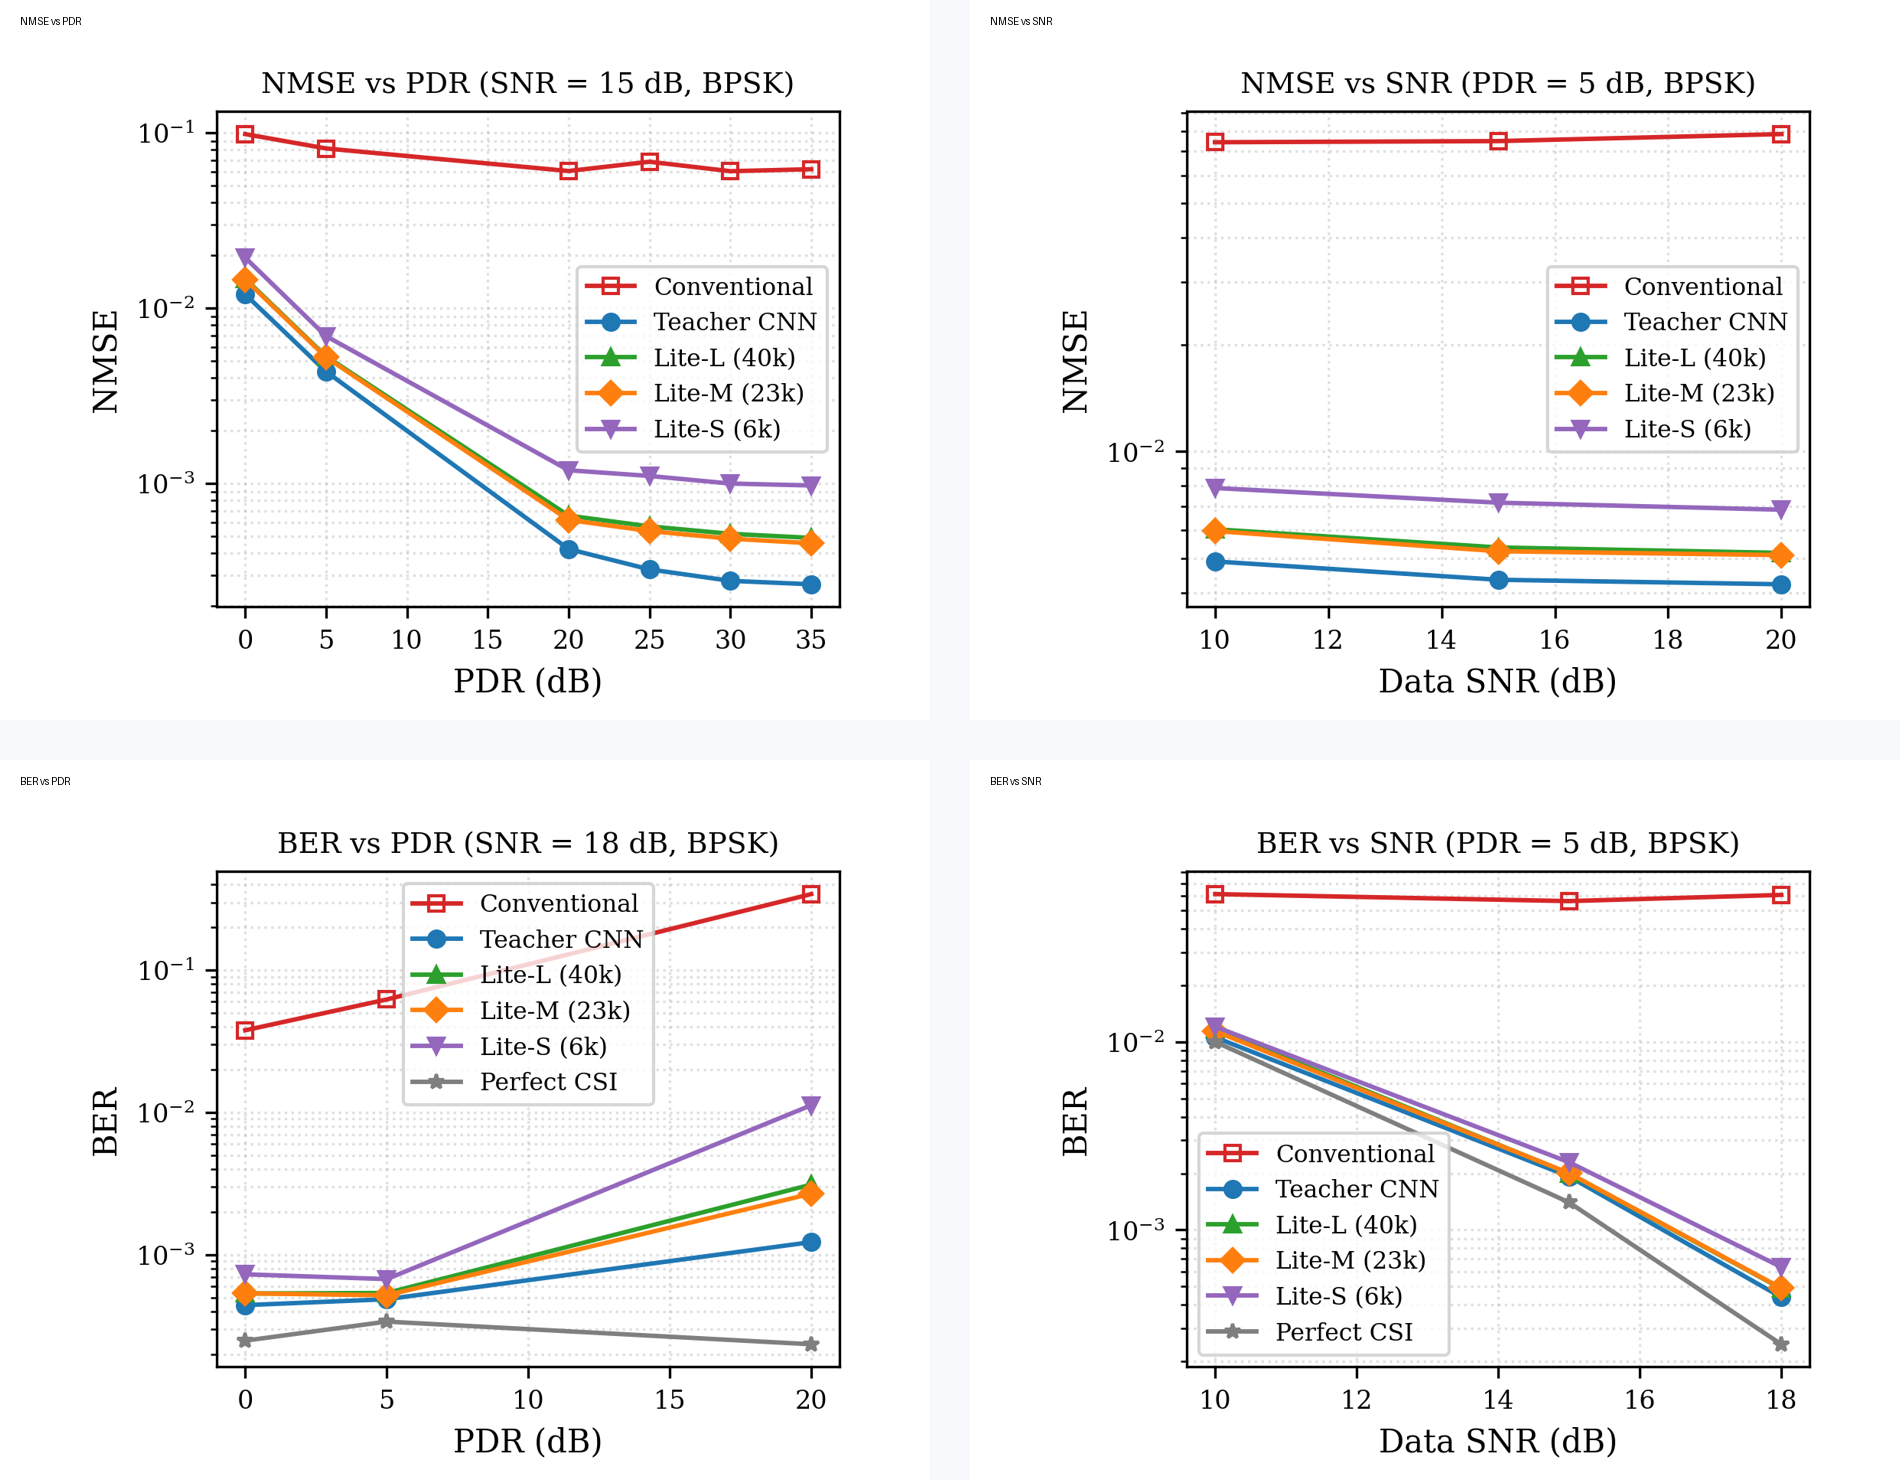
\includegraphics[width=\linewidth]{performance_overview.png}
    \caption{Main performance results for the teacher and distilled students. Lite-M tracks the teacher closely across the retained evaluation suite and is the best overall operating point among the compact models.}
\end{figure}

The most useful representative operating point is PDR = 5\,dB. At that point:
\begin{itemize}
    \item Conventional estimator NMSE is $8.1410\times10^{-2}$ and BER is $6.0666\times10^{-2}$.
    \item Teacher CNN reaches NMSE $4.3520\times10^{-3}$ and BER $4.3899\times10^{-4}$.
    \item \textbf{Lite-M} reaches NMSE $5.2490\times10^{-3}$ and BER $4.9049\times10^{-4}$ with only 22,789 parameters.
\end{itemize}

\begin{table}[H]
\centering
\caption{Key result summary at the representative PDR = 5\,dB operating point.}
\begin{tabular}{lrrr}
\toprule
Method & Params & NMSE & BER \\
\midrule
Conventional & --- & 8.1410e-02 & 6.0666e-02 \\
Teacher CNN & 245,473 & 4.3520e-03 & 4.3899e-04 \\
Lite-L & 40,049 & 5.3068e-03 & 4.8803e-04 \\
\textbf{Lite-M} & \textbf{22,789} & \textbf{5.2490e-03} & \textbf{4.9049e-04} \\
Lite-S & 6,137 & 6.9299e-03 & 6.3518e-04 \\
\bottomrule
\end{tabular}
\end{table}

\subsection{Why Lite-M Is the Final Model}

Lite-L is closest to the teacher, but Lite-M gives the better overall balance. Lite-S is the most aggressive compression point, yet it shows visibly larger degradation under harder conditions. Lite-M is therefore the model that best represents our final contribution:
\begin{itemize}
    \item strong compression: 10.8$\times$ fewer parameters than the teacher,
    \item practical efficiency gain: about 1.9$\times$ measured inference speedup on Apple MPS,
    \item small accuracy gap at practical operating points.
\end{itemize}

\begin{figure}[H]
    \centering
    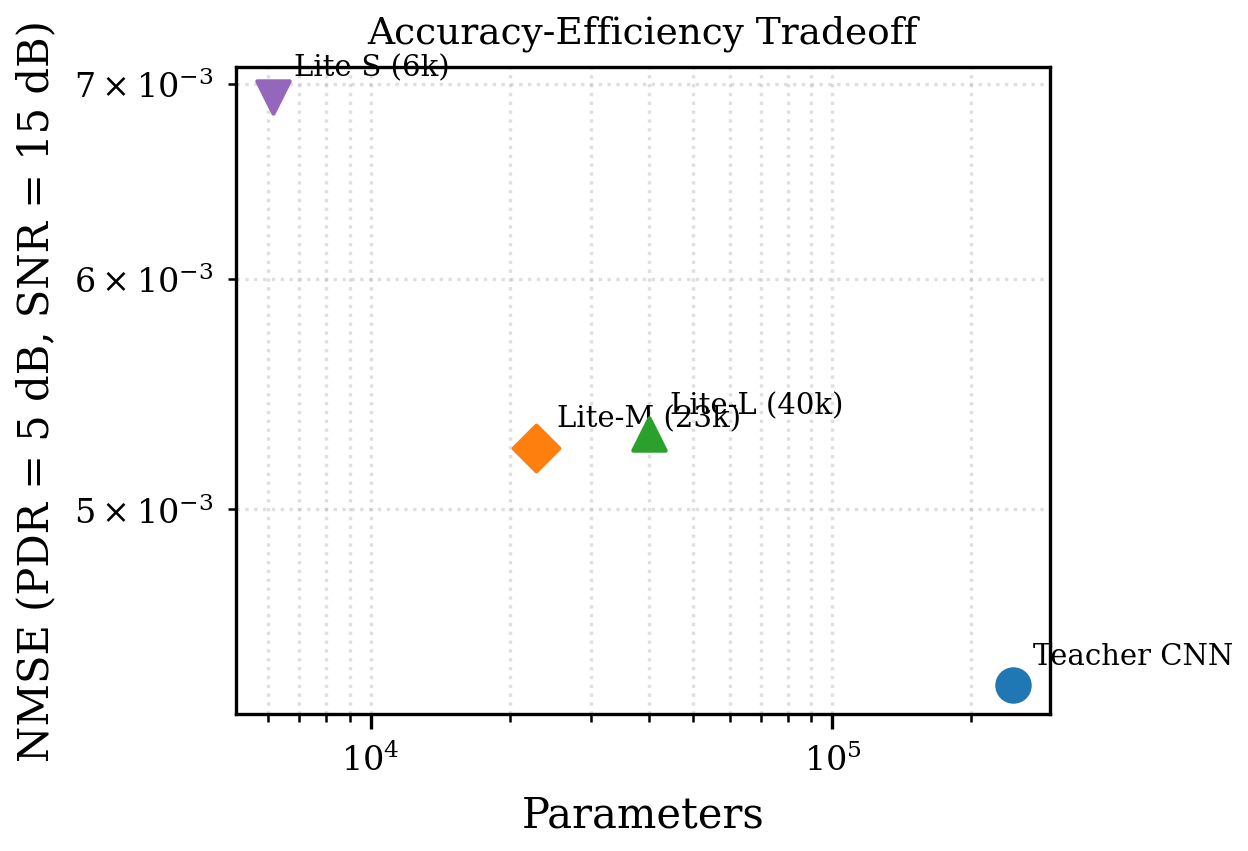
\includegraphics[width=0.77\linewidth]{tradeoff.png}
    \caption{Compression tradeoff. Lite-M is the most balanced point between parameter count and estimation quality.}
\end{figure}

\section{Conclusion and Team Contributions}

\subsection{Conclusion}

This project started from an original Zak-OTFS paper that had no official public code. We first rebuilt the baseline pipeline, including channel simulation, support-domain estimation, CNN refinement, and detector integration. That baseline gave us a trustworthy teacher model and a reproducible evaluation environment.

The main novelty we added is a structural explanation of why compression should work at all. After dechirping, the Zak-OTFS support image is low-dimensional for physical reasons, and this explains why a compact student can imitate a much larger CNN without collapsing in performance. That idea is supported by singular-value analysis, a simple SVD projection baseline, and the final Lite-M results.

The final take-away is clear: \textbf{our contribution is not just a smaller CNN.} It is a structure-aware interpretation of Zak-OTFS support estimation, plus a practical distilled model that leverages that structure well enough to retain most of the teacher's value at much lower complexity.

\subsection{Contribution Split}

To keep the report transparent, the team work is summarized below by responsibility area. Mayank Sharma, Rohit Kumar Mourya, and Jyotiraditya Singh Rathore shared the core technical ownership of the project, while Madhav and Dikshant Jha shared the supporting documentation, validation, and presentation work needed to complete the final deliverables.

\begin{table}[H]
\centering
\caption{Team responsibility split.}
\begin{tabularx}{\linewidth}{>{\bfseries}p{0.18\linewidth}p{0.26\linewidth}X}
\toprule
Roll No. & Name & Primary responsibility areas \\
\midrule
B23ES1023 & Mayank Sharma & End-to-end baseline integration, final novelty positioning, and report consolidation. \\
B23ES1029 & Rohit Kumar Mourya & Experiment execution, result checking, and original-vs-baseline-vs-novelty comparison analysis. \\
B23ES1017 & Jyotiraditya Singh Rathore & Methodology explanation, structural-compressibility writeup, and final technical narrative support. \\
B23ES1021 & Madhav & Figure curation, documentation support, and formatting cleanup for the final report package. \\
B23ES1014 & Dikshant Jha & Validation passes, artifact organization, and presentation-level polishing of the final deliverables. \\
\bottomrule
\end{tabularx}
\end{table}

\keybox{\textbf{Final project message.} Original paper: CNN-aided Zak-OTFS estimation. Our baseline: faithful end-to-end reimplementation. Our novelty: physics-induced support compressibility explains why Lite-M can compress the teacher so effectively.}

\vfill
\begin{center}
{\small References used in this report come from the reproduced project assets, the original Zak-OTFS paper, and the validated final IEEE draft prepared from the same repository.}
\end{center}

\end{document}
